\documentclass[10pt, twocolumn, twoside, letterpaper]{IEEEtran}

\usepackage[activate={true, nocompatibility}, final, tracking=true, kerning=true, spacing=true, factor=1100, stretch=10, shrink=10]{microtype}
\linespread{0.9}

\makeatletter
\def\ps@IEEEtitlepagestyle{
  \def\@oddfoot{\mycopyrightnotice}
  \def\@evenfoot{}
}

\def\mycopyrightnotice{
  {\footnotesize
  \begin{minipage}{\textwidth}
  \centering
  978-1-7281-4164-0/19/\$31.00 \copyright2019 IEEE
  \end{minipage}
  }
}

\ifCLASSINFOpdf
   \usepackage[pdftex]{graphicx}
\else
   \usepackage[dvips]{graphicx}
\fi

\ifCLASSOPTIONcompsoc
  \usepackage[caption=false, font=normalsize, labelfont=sf, textfont=sf]{subfig}
\else
  \usepackage[caption=false, font=footnotesize]{subfig}
\fi

\usepackage{amsmath}
\usepackage{bm}
\usepackage{amssymb}
\usepackage{algorithm}
\usepackage{algorithmic}
\usepackage{stfloats}
\usepackage{url}
\usepackage{siunitx}
\usepackage{fancyref}

\usepackage{geometry}
\geometry{letterpaper, top=0.7in, bottom=0.7in, left=0.65in, right=0.65in}

\usepackage[acronym, nomain]{glossaries}

% Define "long-s" key: 
\glsaddkey* {longs}% key 
{\glsentrylong{\glslabel}s}% default value 
{\glsentrylongs}% command analogous to \glsentrytext 
{\Glsentrylongs}% command analogous to \Glsentrytext 
{\glslongs}% command analogous to \glstext 
{\Glslongs}% command analogous to \Glstext 
{\GLSlongs}% command analogous to \GLStext

%% Define "short-s" key: 
\glsaddkey* {shorts}% key 
{\glsentryshort{\glslabel}s}% default value 
{\glsentryshorts}% command analogous to \glsentrytext 
{\Glsentryshorts}% command analogous to \Glsentrytext 
{\glsshorts}% command analogous to \glstext 
{\Glsshorts}% command analogous to \Glstext 
{\GLSshorts}% command analogous to \GLStext

\DeclareRobustCommand{\glss}[1]
{%
  \ifglsused{#1}{\glsshorts{#1}}{\glslongs{#1} (\glsshorts{#1})\glsunset{#1}}%
}

\DeclareRobustCommand{\Glss}[1]
{%
  \ifglsused{#1}{\Glsshorts{#1}}{\Glslongs{#1} (\glsshorts{#1})\glsunset{#1}}%
}

% Define "long-ing" key: 
\glsaddkey* {longing}% key 
{\glsentrylong{\glslabel}ing}% default value 
{\glsentrylonging}% command analogous to \glsentrytext 
{\Glsentrylonging}% command analogous to \Glsentrytext 
{\glslonging}% command analogous to \glstext 
{\Glslonging}% command analogous to \Glstext 
{\GLSlonging}% command analogous to \GLStext

%% Define "short-ing" key: 
\glsaddkey* {shorting}% key 
{\glsentryshort{\glslabel}ing}% default value 
{\glsentryshorting}% command analogous to \glsentrytext 
{\Glsentryshorting}% command analogous to \Glsentrytext 
{\glsshorting}% command analogous to \glstext 
{\Glsshorting}% command analogous to \Glstext 
{\GLSshorting}% command analogous to \GLStext

\DeclareRobustCommand{\glsing}[1]
{%
  \ifglsused{#1}{\glsshorting{#1}}{\glslonging{#1} (\glsshorting{#1})\glsunset{#1}}%
}

\DeclareRobustCommand{\Glsing}[1]
{%
  \ifglsused{#1}{\Glsshorting{#1}}{\Glslonging{#1} (\glsshorting{#1})\glsunset{#1}}%
}

% Define "long-ed" key: 
\glsaddkey* {longed}% key 
{\glsentrylong{\glslabel}ed}% default value 
{\glsentrylonged}% command analogous to \glsentrytext 
{\Glsentrylonged}% command analogous to \Glsentrytext 
{\glslonged}% command analogous to \glstext 
{\Glslonged}% command analogous to \Glstext 
{\GLSlonged}% command analogous to \GLStext

%% Define "short-ed" key: 
\glsaddkey* {shorted}% key 
{\glsentryshort{\glslabel}ed}% default value 
{\glsentryshorted}% command analogous to \glsentrytext 
{\Glsentryshorted}% command analogous to \Glsentrytext 
{\glsshorted}% command analogous to \glstext 
{\Glsshorted}% command analogous to \Glstext 
{\GLSshorted}% command analogous to \GLStext

\DeclareRobustCommand{\glsed}[1]
{%
  \ifglsused{#1}{\glsshorted{#1}}{\glslonged{#1} (\glsshorted{#1})\glsunset{#1}}%
}

\DeclareRobustCommand{\Glsed}[1]
{%
  \ifglsused{#1}{\Glsshorted{#1}}{\Glslonged{#1} (\glsshorted{#1})\glsunset{#1}}%
}

\newacronym{1D}{1D}{$1$-Dimensional}
\newacronym{2D}{2D}{$2$-Dimensional}
\newacronym{3D}{3D}{$3$-Dimensional}
\newacronym[longs={$3$-Dimensional Point Clouds}, shorts={3DPCs}]{3DPC}{3DPC}{$3$-Dimensional Point Cloud}
\newacronym{4D}{4D}{$4$-Dimensional}
\newacronym{4DCT}{4DCT}{$4$-Dimensional Computed Tomography}
\newacronym[longs={Attenuation Corrected Motion Compensated Image Reconstructions}, shorts={ACMCIRs}, longing={Attenuation Corrected Motion Compensated Image Reconstructing}, shorting={ACMCIRing}, longed={Attenuation Corrected Motion Compensated Image Reconstructed}, shorted={ACMCIRed}]{ACMCIR}{ACMCIR}{Attenuation Corrected Motion Compensated Image Reconstruct}
\newacronym[longs={Attenuation Corrections}, shorts={ACs}, longing={Attenuation Correcting}, shorting={ACing}, longed={Attenuation Corrected}, shorted={ACed}]{AC}{AC}{Attenuation Correct}
\newacronym[longs={Affine Deformations}, shorts={ADs}, longing={Affine Deforming}, shorting={ADing}, longed={Affine Deformed}, shorted={ADed}]{AD}{AD}{Affine Deformation}
\newacronym{AP}{AP}{Anterior Posterior}
\newacronym{ATP}{ATP}{Adenosine Triphosphate}
\newacronym[longs={B-Splines}, shorts={BSs}, longing={B-Splining}, shorting={BSing}, longed={B-Splined}, shorted={BSed}]{BS}{BS}{B-Spline}
\newacronym[longs={Cross Correlations}, shorts={CCs}, longing={Cross Correlating}, shorting={CCing}, longed={Cross Correlated}, shorted={CCed}]{CC}{CC}{Cross Correlation}
\newacronym{CCT}{CCT}{Cine Computed Tomography}
\newacronym{CG}{CG}{Conjugate Gradient}
\newacronym{COM}{COM}{Centre of Mass}
\newacronym[longs={Control Points}, shorts={CPs}]{CP}{CP}{Control Point}
\newacronym[longs={Control Point Grids}, shorts={CPGs}]{CPG}{CPG}{Control Point Grid}
\newacronym{CT}{CT}{Computed Tomography}
\newacronym{DD}{DD}{Data Driven}
\newacronym{DDG}{DDG}{Data Driven Gating}
\newacronym[longs={Deformation Vector Fields}, shorts={DVFs}]{DVF}{DVF}{Deformation Vector Field}
\newacronym{EANM}{EANM}{European Association of Nuclear Medicine}
\newacronym{EM}{EM}{Expectation Maximisation}
\newacronym{FDG}{FDG}{Fludeoxyglucose}
\newacronym{F-FDG}{F-FDG}{Fluorine-$18$ Fludeoxyglucose}
\newacronym[longs={Fields of View}, shorts={FOVs}]{FOV}{FOV}{Field Of View}
\newacronym{FWHM}{FWHM}{Full Width at Half Maximum}
\newacronym{GD}{GD}{Gradient Descent}
\newacronym{GE}{GE}{General Electric}
\newacronym[longs={Ground Truths}, shorts={GTs}]{GT}{GT}{Ground Truth}
\newacronym[longs={Hounsfield Units}, shorts={HUs}]{HU}{HU}{Hounsfield Unit}
\newacronym[longs={Image Registrations}, shorts={IRs}, longing={Image Registering}, shorting={IRing}, longed={Image Registered}, shorted={IRed}]{IR}{IR}{Image Registration}
\newacronym[longs={Kilo Becquerel per Millilitres}, shorts={KBq/mLs}]{KBq/mL}{KBq/mL}{Kilo Becquerel per Millilitre}
\newacronym[longs={Kilo Electron Volts}, shorts={KeVs}]{KeV}{KeV}{Kilo Electron Volt}
\newacronym[longs={Kilo Volt}, shorts={KVs}]{KV}{KV}{Kilo Volt}
\newacronym[longs={Light Emitting Diodes}, shorts={LEDs}]{LED}{LED}{Light Emitting Diode}
\newacronym[longs={Lines of Responce}, shorts={LORs}]{LOR}{LOR}{Line of Response}
\newacronym[longs={Mean Absolute Errors}, shorts={MAEs}]{MAE}{MAE}{Mean Absolute Error}
\newacronym{MAPE}{MAPE}{Mean Absolute Percentage Error}
\newacronym{MBF}{MBF}{Myocardial Blood Flow}
\newacronym[longs={Motion Compensated Image Reconstructions}, shorts={MCIRs}, longing={Motion Compensated Image Reconstructing}, shorting={MCIRing}, longed={Motion Compensated Image Reconstructed}, shorted={MCIRed}]{MCIR}{MCIR}{Motion Compensated Image Reconstruction}
\newacronym[longs={Motion Compensated Images}, shorts={MCIs}]{MCI}{MCI}{Motion Compensated Image}
\newacronym[longs={Motion Corrections}, shorts={MCs}, longing={Motion Correcting}, shorting={MCing} longed={Motion Corrected}, shorted={MCed}]{MC}{MC}{Motion Correction}
\newacronym{MI}{MI}{Mutual Information}
\newacronym{ML}{ML}{Maximum Likelihood}
\newacronym{MLAA}{MLAA}{Maximum Likelihood Reconstruction of Activity and Attenuation}
\newacronym{MLE}{MLE}{Maximum Likelihood Estimation}
\newacronym{MLEM}{MLEM}{Maximum Likelihood Expectation Maximisation}
\newacronym[longs={Motion Models}, shorts={MMs}, longing={Motion Modelling}, shorting={MMing}, longed={Motion Modelled}, shorted={MMed}]{MM}{MM}{Motion Model}
\newacronym[longs={Myocardial Perfusion Images}, shorts={MPIs}, longing={Myocardial Perfusion Imaging}, shorting={MPIing}, longed={Myocardial Perfusion Imaged}, shorted={MPIed}]{MPI}{MPI}{Myocardial Perfusion Image}
\newacronym{MR}{MR}{Magnetic Resonance}
\newacronym[longs={Mean Squared Errors}, shorts={MSEs}]{MSE}{MSE}{Mean Squared Error}
\newacronym[longs={Attenuation Maps}, shorts={Mu-Maps}]{Mu-Map}{Mu-Map}{Attenuation Map}
\newacronym[longs={Naive Attenuation Corrected Reconstructions}, shorts={NACRs}, longing={Naive Attenuation Corrected Reconstructing}, shorting={NACRing}, longed={Naive Attenuation Corrected Reconstructed}, shorted={NACRed}]{NACR}{NACR}{Naive Attenuation Corrected Reconstruct}
\newacronym[longs={Non-Attenuation Corrections}, shorts={NACs}, longing={Non-Attenuation Correcting}, shorting={NACing}, longed={Non-Attenuation Corrected}, shorted={NACed}]{NAC}{NAC}{Non-Attenuation Correct}
\newacronym{NMI}{NMI}{Normalised Mutual Information}
\newacronym{ND}{ND}{$n$-Dimensional}
\newacronym[longs={Non-Rigid Deformations}, shorts={NRDs}, longing={Non-Rigid Deforming}, shorting={NRDing}, longed={Non-Rigid Deformed}, shorted={NRed}]{NRD}{NRD}{Non-Rigid Deformation}
\newacronym{NTOF}{NTOF}{Non-Time of Flight}
\newacronym{OSEM}{OSEM}{Ordered Subset Expectation Maximisation}
\newacronym[longs={Principal Components}, shorts={PCs}]{PC}{PC}{Principal Component}
\newacronym{PCA}{PCA}{Principal Component Analysis}
\newacronym{PET}{PET}{Positron Emission Tomography}
\newacronym{PSMA}{PSMA}{Prostate Specific Membrane Antigen}
\newacronym[longs={Respiratory Correspondence Models}, shorts={RCMs}, longing={Respiratory Correspondence Modelling}, shorting={RCMing}, longed={Respiratory Correspondence Modelled}, shorted={RCMed}]{RCM}{RCM}{Respiratory Correspondence Model}
\newacronym[longs={Rigid Deformations}, shorts={RDs}, longing={Rigid Deforming}, shorting={RDing}, longed={Rigid Deformed}, shorted={RDed}]{RD}{RD}{Rigid Deformation}
\newacronym{RDP}{RDP}{Relative Difference Prior}
\newacronym[longs={Respiratory Motions}, shorts={RMs}]{RM}{RM}{Respiratory Motion}
\newacronym[longs={Regions of Interest}, shorts={ROIs}]{ROI}{ROI}{Region of Interest}
\newacronym{RPM}{RPM}{Real Time Position Management}
\newacronym{SGD}{SGD}{Stochastic Gradient Descent}
\newacronym{SI}{SI}{Superior Inferior}
\newacronym{SIRF}{SIRF}{Synergistic Image Reconstruction Framework}
\newacronym[longs={Signal to Noise Ratios}, shorts={SNRs}]{SNR}{SNR}{Signal to Noise Ratio}
\newacronym[longs={Surrogate Signals}, shorts={SSs}]{SS}{SS}{Surrogate Signal}
\newacronym{SSD}{SSD}{Sum of Squared Differences}
\newacronym{STIR}{STIR}{Software for Tomographic Image Reconstruction}
\newacronym[longs={Standard Uptake Values}, shorts={SUVs}]{SUV}{SUV}{Standard Uptake Value}
\newacronym{SVD}{SVD}{Singular Value Decomposition}
\newacronym{TOF}{TOF}{Time of Flight}
\newacronym[longs={Thin Plate Splines}, shorts={TPSs}]{TPS}{TPS}{Thin Plate Spline}
\newacronym{XCAT}{XCAT}{$4$-Dimensional Extended Cardiac Torso}

\newcommand{\cmmnt}[1]{\@bsphack\@esphack}

\usepackage[style=ieee, doi=false, isbn=false, url=false, maxbibnames=1, minbibnames=1, maxcitenames=1, mincitenames=1, backend=biber, defernumbers=false]{biblatex}
\addbibresource{./bibtex/bib/Biblio.bib}

\IEEEpubid{\begin{minipage}{\textwidth}\ \\[9pt] \centering
\medskip
\\
978-1-7281-2260-1/19/\$31.00~\copyright~2019~IEEE
\end{minipage}}

\begin{document}
\title{PET/CT Respiratory Motion Correction Using NAC Derived Deformation Fields to Warp and Attenuation Correct With a Single Attenuation Map}

\pagestyle{plain}
\pagenumbering{gobble}

\author{Alexander~C.~Whitehead,~\IEEEmembership{Student~Member,~IEEE,}
        Nikos~Efthimiou,~\IEEEmembership{Member~IEEE},
        Scott~W.~Wollenweber,~\IEEEmembership{Senior~Member~IEEE,}
        Charles~W.~Stearns,~\IEEEmembership{Fellow,~IEEE,}
        Brian~F.~Hutton,~\IEEEmembership{Senior~Member,~IEEE,}
        Jamie~R.~McClelland
        and~Kris~Thielemans,~\IEEEmembership{Senior~Member,~IEEE}%

    \thanks{Alexander~C.~Whitehead, Brian~F.~Hutton and Kris~Thielemans are with the Institute of Nuclear Medicine, University College London, London, NW1~2BU, UK (contact: \texttt{alexander.whitehead.18@ucl.ac.uk}).}%
    \thanks{Nikos~Efthimiou is with .}%
    \thanks{Alexander~C.~Whitehead and Jamie~R.~McClelland are with the Centre for Medical Image Computing, University College London, London, NW1~2BU, UK.}%
    \thanks{Scott~Wollenweber and Charles~Stearns are with Molecular Imaging \& Computed Tomography Engineering, GE Healthcare, USA}%
    \thanks{This research is supported by GE Healthcare, the NIHR UCLH Biomedical Research Centre and the EPSRC-funded UCL Centre for Doctoral Training in Medical Imaging (EP/L016478/1). The software used was partly produced by the Computational Collaborative Project in Synergistic PET-MR Reconstruction, CCP PET-MR, UK EPSRC grant EP/M022587/1.}%
    \thanks{Jamie~R.~McClelland is supported by a Cancer Research UK Centres Network Accelerator Award Grant (A21993) to the ART-NET consortium and a CRUK Multi-disciplinary grant (CRC 521).}%
}

\maketitle
\IEEEpeerreviewmaketitle

\begin{abstract}
    What to do about the problem of attenuation correction is a difficult decision to make while implementing a motion correction algorithm in positron emission tomography. It could be corrected for; which may introduce an unwanted bias (through misaligned anatomy) into the motion correction algorithm or increase dose to the patient. It could also not be corrected for; which makes finding an optimal solution to motion correction much more difficult (by introducing an uncertainty into the activity distribution thus making anatomy more indiscernible). This work proposes a compromise, it builds upon previous work which suggested that non-attenuation corrected data was suitable for motion correction (of intra-respiratory cycle motion), through the use of motion models, if time of flight data is available. Here, the previous work is expanded upon by first validating the method on inter-respiratory cycle motion before reincorporating attenuation correction. Phantom simulations are used, for one bed position, with a field of view including the base of the lungs and the diaphragm. Non-attenuation corrected volumes are reconstructed using ordered subset expectation maximisation and used as input for motion model estimation. A single attenuation map is then warped to the volumes, using the motion model, and the volumes are attenuation corrected. The output from this method is then evaluated against a clinical reconstruction of the same data using both a visual and standardised uptake value analysis as well as a comparison of a profile over the volume. Results indicate that not only is motion correction of inter-respiratory cycle motion possible, with this method, but it is also suitable to incorporate attenuation correction without negatively impacting the solution found. The implications for future research include the possibility of directly incorporating the motion model estimation into the reconstruction algorithm as well as also attempting to simultaneously estimate deformations for the attenuation map as well as the activity distribution.
\end{abstract}

\section{Introduction} \label{sec:introduction}
    \IEEEPARstart{R}{espiratory} motion reduces image resolution in \gls{PET} by introducing blurring and misalignment artefacts~\cite{Nehmeh2008a}. Unless gated \gls{CT} are available (which themselves increase dose to the patient), to avoid mis-registration due to attenuation mismatches, most existing \gls{MC} methods rely on pair-wise registration of gated \gls{NAC} \gls{PET} volumes~\cite{LungMotionDiaphragmBaiBib}~\cite{Oliveira2014}. This is a challenging problem due to the low contrast and high noise of these volumes.
    
    \glsing{MM} approaches \gls{MC} by fitting a \glss{RCM} on the \glss{DVF} which would deform a \glsed{MCIR} volume (at the mean respiratory position) to each input bin and on the \gls{SS} value for that bin. Thus for any given \gls{SS} value the \gls{RCM} could return a \gls{DVF} to warp either from or to the mean position to the bin at that \gls{SS} value~\cite{McClelland2017}.
    
    Previous work has investigated the possibility of using \glsing{MM} for respiratory \gls{MC} in \gls{NAC} \gls{PET}, and in particular whether incorporating \gls{TOF} information increases the validity of the \gls{MC} potential derived from the \gls{NAC} reconstructed volumes. It was found that \gls{NAC} \gls{TOF} \gls{PET} was suitable to \gls{MC} data without inter-respiratory cycle variation~\cite{Whitehead2019ImpactPET}. It is an aim of this work to determine if \gls{NAC} \gls{TOF} data is sufficient to model more complex inter-respiratory cycle motion.
    
    \gls{NAC} volumes are not particularly clinically useful as they are not an accurate representation of the distribution of activity in the patient, therefore they are not quantitative. Is is also an aim of this work to determine if \gls{NMI} pair-wise registration of a \glsed{MCIR} volume (at the mean respiratory position) and a \gls{Mu-Map} (from any position) and then warping this \gls{Mu-Map} (now at the mean respiratory position) back to the bins which generated the \gls{MCIR} volume for \gls{ACMCIR} is viable.

\section{Methods} \label{sec:methods}
    \subsection{XCAT Volume Generation} \label{sec:xcat_volume_generation}
        \gls{XCAT}~\cite{Segars2010} was used to generate both $6$ volumes over a single linear \SI{5}{\second} breathing cycle from \gls{XCAT} (henceforth referred to as simple data) and $240$ volumes over a more complex (with inter-respiratory cycle variation) \SI{120}{\second} breathing cycle derived from a respiratory trace captured using an \gls{RPM} (henceforth referred to as complex data). The simple data contained both a volume at full expiration at the beginning of the cycle as well as at the end of the cycle. Both data used max displacement settings for the extent of \gls{AP} and \gls{SI} motion of \SI{1.2}{\centi\metre} and \SI{2.0}{\centi\metre} respectively. Activity concentrations were derived from a static \gls{FDG} patient scan. The \gls{FOV} included the base of the lungs, diaphragm and the top of the liver with a \SI{20}{\milli\metre} diameter spherical lesion placed into the centre of the right lung.
    
    \subsection{PET Acquisition Simulation} \label{sec:pet_acquisition_simulation}
        \gls{PET} acquisitions were simulated (and reconstructed) using \gls{STIR}~\cite{Thielemans2012, Efthimiou2018} through \gls{SIRF}~\cite{Ovtchinnikov2017, Ovtchinnikov2019CCPPETMRSIRF} to forward project the data using the geometry of a \gls{GE} Discovery 710 with a \gls{TOF} resolution of \SI{375}{\pico\second}. This \gls{TOF} resolution is similar to the \gls{GE} Signa \gls{PET}/\gls{MR}, however, \gls{TOF} mashing is used to reduce computation time resulting in $13$ \gls{TOF} time bins of size \SI{376.5}{\pico\second}). Attenuation was included, in the simulation, using the relevant \gls{Mu-Map} generated by \gls{XCAT}. Scatter and randoms were not taken into account. Multiple noise realisations were generated to simulate an acquisition over \SI{120}{\second}, emulating a standard single bed position acquisition. The simple data was 'pseudo gated', by using noise realisations which (when applied) resulted in as if it had been gated into $6$ bins. The complex data was simulated with realistic noise realisations and then programmatically gated, into $10$ bins, based on a respiratory \gls{SS}. A respiratory \gls{SS} was generated for both sets of data using static \gls{PCA}~\cite{Thielemans2011}. \gls{SS} values were ascertained for the post-gated data by taking an average of the \gls{SS} values of the data in each bin.
    
    \subsection{Non-Attenuation Corrected Image Reconstruction} \label{sec:non-attenuation_corrected_image_reconstruction}
        Data were initially reconstructed without \gls{AC} using \gls{OSEM} with $2$ full iterations and $24$ subsets~\cite{Hudson1994}. Volumes were post-filtered using a Gaussian blur with a kernel size of \SI{6.4}{\milli\metre} \gls{FWHM}.
    
    \subsection{Motion Model Estimation} \label{sec:motion_model_estimation}
        For each data set \gls{3D} B-spline interpolated \glss{DVF} were used to model spatial deformations. A generalised framework unifying \gls{IR} and respiratory \glss{MM}, NiftyRegResp, was used to estimate \glss{RCM} and \glss{MCIR}~\cite{McClelland2017}. \gls{SSD} was used as the objective function and the second order derivative of the \gls{DVF} was used as a penalty. The \gls{CPG} spacing of the \gls{DVF} and penalty weight were tuned using a grid search.
    
    \subsection{Attenuation Map Warping} \label{sec:attenuation_map_warping}
        A \gls{Mu-Map} was selected randomly from the \glss{Mu-Map} generated by \gls{XCAT} for both data sets, this \gls{Mu-Map} was then registered to the \gls{MCIR} generated while fitting the \gls{RCM} from~\Fref{sec:motion_model_estimation}. A \gls{NMI} registration was used to accomplish this with parameters selected using a grid search. The \gls{RCM} was then used to generate \gls{DVF} for the \gls{SS} values of each bin and use this to warp the \gls{Mu-Map} from the mean respiratory position to each bin.
        
    \subsection{Attenuation Corrected Motion Corrected Image Reconstruction} \label{sec:attenuation_corrected_image_reconstruction}
        Data were re-reconstructed with \gls{AC} using the \glss{Mu-Map} from~\Fref{sec:attenuation_map_warping}. The same reconstruction parameters as in~\Fref{sec:attenuation_corrected_image_reconstruction} were used. This data was then motion corrected again as in~\Fref{sec:motion_model_estimation} to generate a final \gls{AC} \gls{MCIR}. This is referred to as \gls{ACMCIR}.
    
    \subsection{Evaluation} \label{sec:evaluation}
        To evaluate the validity of the \glsing{MM} results the \gls{COM} of the lesion, over time, was tracked for both \gls{NAC} and \gls{AC} reconstructions of both data sets. This was achieved by warping a volume only including the lesion in the reference position, and then computing its \gls{COM}.
        
        In addition to the reconstructions performed in~\Fref{sec:attenuation_corrected_image_reconstruction} data were also reconstructed by simply summing all gates together and using one randomly positioned \gls{Mu-Map} for \gls{AC}, this process matches current clinical practise. Here, this is referred to as \gls{NACR}. The data from this, more naive, approach was used for each data set to evaluate the improvement that the new method afforded. The comparisons used included; a visual analysis, a profile over the lesion and \gls{SUV}\textsubscript{max}, \gls{SUV}\textsubscript{median} and \gls{SUV}\textsubscript{peak}. \gls{SUV}\textsubscript{peak} here was defined following \gls{EANM} guidelines~\cite{Boellaard2015FDG2.0}

\section{Results} \label{sec:results}
    \begin{figure}
        \centering
        \subfloat[][]{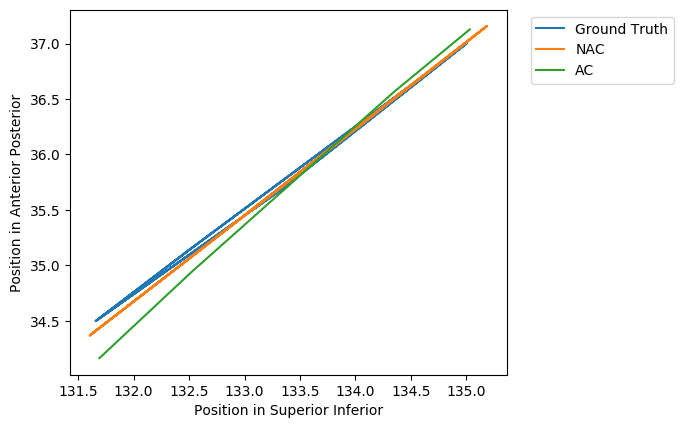
\includegraphics[width=0.5\linewidth]{figures/one_com.png}}
        \subfloat[][]{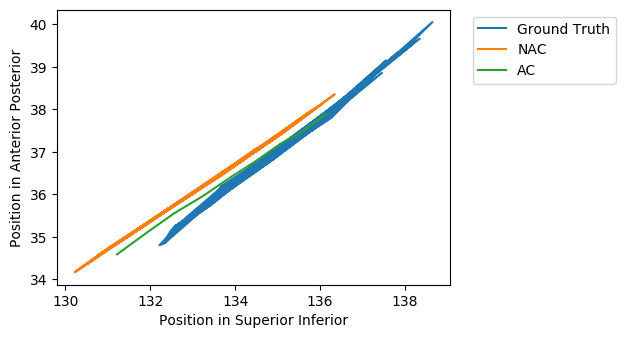
\includegraphics[width=0.5\linewidth]{figures/anon_com.png}}
        \captionsetup{singlelinecheck=false, justification=centering}
        \caption{The path of the \gls{COM} of the lesion. Horizontal (respectively vertical) axis corresponds to motion in the \gls{AP} (respectively \gls{SI}) direction over the simple data for (a) and the complex data for (b). Different curves denote \gls{COM} displacement for  ground truth data, the estimated data from the \gls{NAC} based \gls{RCM} and the estimated data from the \gls{AC} based \gls{RCM}.}
        \label{fig:com}
    \end{figure}
    
    \gls{COM} results can be seen in~\Fref{fig:com}, the \gls{COM} of both the \gls{NAC} and \gls{AC} for both the simple and complex data relatively closely matches the ground truth \gls{COM}.
    
    \begin{figure*}
        \centering
        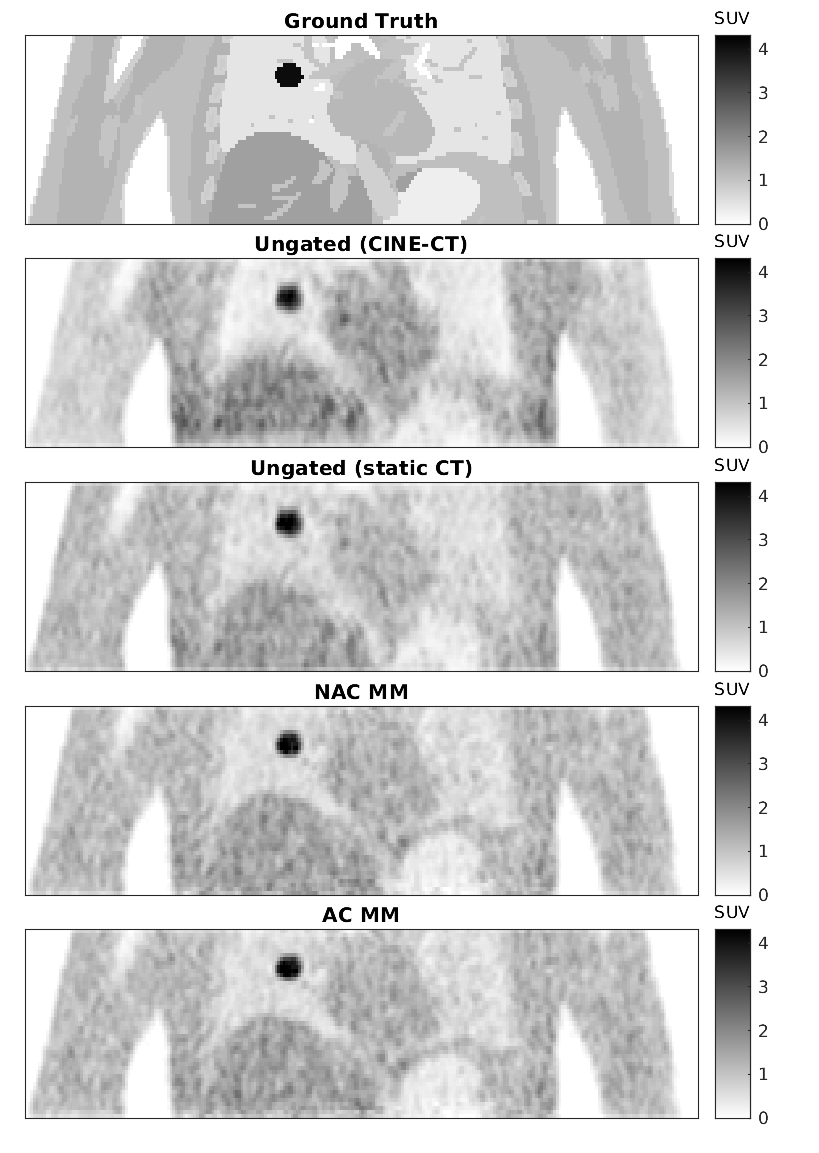
\includegraphics[width=1.0\linewidth]{figures/visual_analysis.png}
        \captionsetup{singlelinecheck=false, justification=centering}
        \caption{First row from left to right: \glsed{NACR} and \glsed{ACMCIR} simple data. Colour map ranges are consistent for all images on this row. Second row: \glsed{NACR} and \glsed{ACMCIR} complex data. Colour map ranges are consistent for all images on this row.}
        \label{fig:visual_analysis}
    \end{figure*}
    
    \begin{figure}
        \centering
        \subfloat[][]{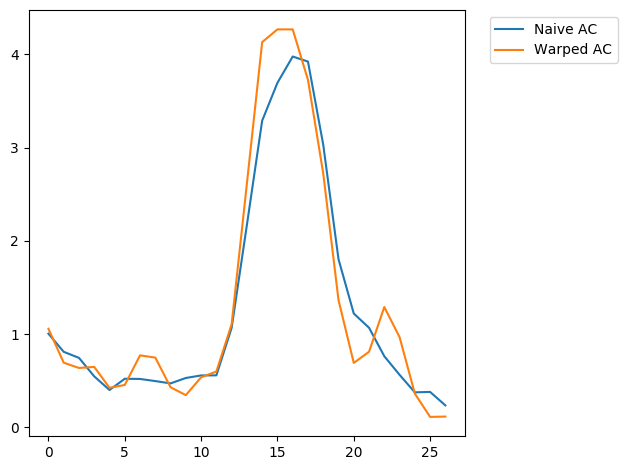
\includegraphics[width=0.5\linewidth]{figures/one_profile.png}}
        \subfloat[][]{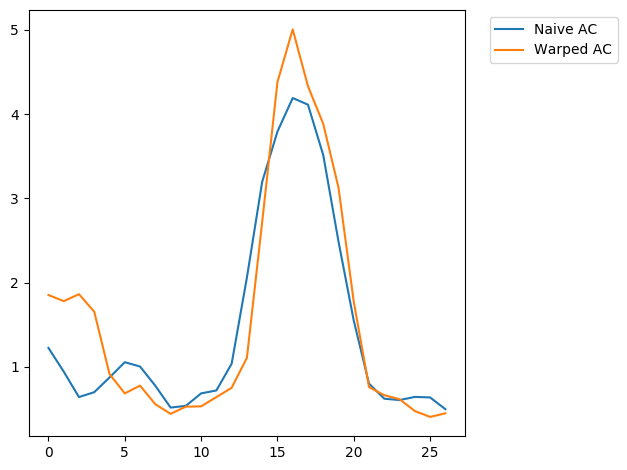
\includegraphics[width=0.5\linewidth]{figures/anon_profile.png}}
        \captionsetup{singlelinecheck=false, justification=centering}
        \caption{A profile across the lesion of the simple data for (a) and the complex data for (b). Each sub-figure shows the profile for both the \gls{NACR} as well as for the \gls{ACMCIR}.}
        \label{fig:profile}
    \end{figure}
    
    \begin{table}
        \centering
        \captionsetup{singlelinecheck=false, justification=centering}
        \caption{Comparison of \gls{SUV}\textsubscript{max}, \gls{SUV}\textsubscript{median} and \gls{SUV}\textsubscript{peak} between the \glsed{NACR} data and the \glsed{ACMCIR} data for both the simple and complex data, plus the difference between \gls{NACR} and \gls{ACMCIR} \glss{SUV} for each data set.}
        
        \resizebox*{1.0\linewidth}{!}
        {
            \begin{tabular}{||c|ccc||}
                \hline
                \textbf{\gls{SUV}} & \textbf{Max} & \textbf{Median} & \textbf{Peak} \\
                \hline
                \textbf{Simple \gls{NACR}}      & $5.40$ & $3.03$ & $3.73$ \\
                \textbf{Simple \gls{ACMCIR}}    & $6.71$ & $3.50$ & $4.07$ \\
                \hline
                \textbf{Simple Difference}      & $1.31$ & $0.47$ & $0.34$ \\
                \hline
                \textbf{Complex \gls{NACR}}     & $4.44$ & $2.93$ & $3.39$ \\
                \textbf{Complex \gls{ACMCIR}}   & $5.00$ & $3.08$ & $3.83$ \\
                \hline
                \textbf{Complex Difference}     & $0.56$ & $0.15$ & $0.44$ \\
                \hline
            \end{tabular}
        }
        \label{tab:suv}
    \end{table}
    
     The \glsed{NACR} data and the \glsed{ACMCIR} data can be seen in~\Fref{fig:visual_analysis}. When compared visually structures can be seen in the \glsed{ACMCIR} data that cannot be seen in the \glsed{NACR} data. For instance, structures at the boundary between the diaphragm and the lung. Additionally, the boundary between the lesion and the lung appears to be sharper and the lesion itself more homogeneous, this can be observed in the profile across the lesion in~\Fref{fig:profile}. \gls{SUV} results can be seen in~\Fref{tab:suv} and consistently show that \glss{SUV} are greater for \gls{ACMCIR} over \gls{NACR} for both simple and complex data.

\section{Discussion and Conclusions} \label{sec:discussion_and_conclusions}
    \glss{MM} derived from \gls{NAC} \and \gls{AC} volumes for both data containing intra and inter-respiratory cycle motion were found to be relatively robust when comparing \gls{COM}. Results from both a visual analysis and from a comparison of profiles and \glss{SUV} shows that \gls{ACMCIR} provides volumes freer from blurring and not as susceptible to artefacts when compared to current clinical practise (\gls{NACR}).
    
    In the future, research will focus on more complex methods of incorporating, directly, both \glsed{MC} \glss{Mu-Map} and \glsing{MM} into reconstruction.

\AtNextBibliography{\scriptsize}
\printbibliography

\end{document}
